\documentclass{article}
\usepackage{multicol}

\title{Deep Blockchains}
\author{Sourabh Niyogi, Michael Chung and Rodney Witcher\\Wolk Inc.\\
{\tt \{sourabh,michael,rodney\}@wolk.com}}
\date{July 10, 2018}

\usepackage{url}
\usepackage{amsfonts}
\usepackage{geometry}
\usepackage{graphicx}
\usepackage{amsmath}
\usepackage[latin1]{inputenc}
\usepackage{tikz}
\usepackage{hyperref}
\hypersetup{
    colorlinks=true,
    linkcolor=blue,
    filecolor=magenta,      
    urlcolor=cyan,
}
\usepackage[nottoc]{tocbibind}
\geometry{left=.75in,top=.75in,right=.75in,bottom=1.0in}


\usepackage{listings}
\usepackage{listings-golang} % import this package after listings
\usepackage{color}

\lstset{ % add your own preferences
    frame=single,
    basicstyle=\footnotesize,
    keywordstyle=\color{red},
    numbers=left,
    numbersep=5pt,
    showstringspaces=false, 
    stringstyle=\color{blue},
    tabsize=4,
    language=Golang % this is it !
}


% Define block styles
\tikzstyle{decision} = [diamond, draw, fill=blue!20, 
    text width=4.5em, text badly centered, node distance=3cm, inner sep=0pt]
\tikzstyle{block} = [rectangle, draw, fill=blue!20, 
    text width=5em, text centered, minimum height=4em]
\tikzstyle{blockchain2} = [rectangle, draw, fill=yellow!50!green, 
    text width=5em, text centered, minimum height=4em]
\tikzstyle{blockchain3} = [rectangle, draw, fill=yellow!90, 
    text width=5em, text centered, minimum height=4em]
\tikzstyle{line} = [draw, -latex']
\tikzstyle{cloud} = [draw, ellipse,fill=red!20, node distance=3cm,
    minimum height=2em]
    
    
\usetikzlibrary{shapes,arrows}


\newcommand{\block}[2]{B^{#1}_{#2}} 
\newcommand{\blockhash}[2]{b^{#1}_{#2}} 
\newcommand{\blockchainstatetransition}[1]{\Upsilon^{i}} 
\newcommand{\blockfinalizationstatetransition}[1]{\Omega^#1} 
\newcommand{\blockstatetransition}[1]{\Pi^#1} 
\newcommand{\submission}[1]{\Lambda^{#1}}  
\newcommand{\statetransition}[2]{\sigma_{#2}^#1} 
\newcommand{\transaction}[2]{T_{#2}^#1} 
\newcommand{\anchortransaction}[2]{\tilde{T}_{#2}^#1} 
\newcommand{\databaseencryptionkey}{\pi} 
\newcommand{\owner}{O} 
\newcommand{\recipient}{R} 
\newcommand{\signature}{\omega} 
\newcommand{\spent}{\phi} 
\newcommand{\keyroot}{\kappa} 
\newcommand{\allowance}{\gamma} 
\newcommand{\defh}[1]{d(#1)} 

\newcommand{\hash}[1]{H(#1)} 
\newcommand{\transactionroot}[2]{\theta_{#2}^#1} 
\newcommand{\tokenroot}[1]{\tau_{#1}} 
\newcommand{\retrieval}[1]{\Xi^{#1}} 
\newcommand{\proofBits}{\texttt{proofBits}}
\newcommand{\proofBytes}{\texttt{proofBytes}}
\newcommand{\submitblock}[2]{\texttt{submitBlock}(#2, #1)}
\newcommand{\startexit}{\texttt{startExit}}
\newcommand{\withdrawoperator}{\texttt{withdrawoperator}}
\newcommand{\encrypt}[1]{encrypt(#1, \databaseencryptionkey)}
\newcommand{\decrypt}[1]{decrypt(#1, \databaseencryptionkey)}
\newcommand{\balance}{\beta}
\newcommand{\emptyhash}{0}
\newcommand{\sql}[1]{\texttt{#1}} 
\newcommand{\json}[1]{\{\texttt{#1}\}} 

\newcommand{\maxstoragecost}{\Omega}
\newcommand{\seedhash}{\gamma}
\newcommand{\seed}{\nu}

\begin{document}
\maketitle

\begin{abstract}
We describe how a {\em deep blockchain} architecture can address bottlenecks of a modern single-layer blockchain without sacrificing their core benefits of immutability, security, or trustlessness.  Fundamentally, this is achievable with higher layer blockchains submitting {\em anchor transactions} which summarize the higher layer's block for inclusion in blocks of the lower layer blockchain, thus making all higher layer blockchains supervenient on lower level blockchain features.   We describe, in particular, a 3-layer blockchain for provable storage and bandwidth in detail: (I) Layer 1 is MainNet, which stores both (a) registered Layer 3 blockchain roots and (b) Layer 2 Block Merkle roots; (II) Layer 2 is a Plasma Cash chain, storing (a) Plasma tokens redeemable for bandwidth and (b) Layer 3 Block hashes; (III) Layer 3 blockchains are any number of blockchains using storage and bandwidth of Layer 2, e.g those that package NoSQL / SQL transactions for typical database operations;  Layers 2 utilizes a Cloudstore abstraction to store and retrieve Layer 2 and Layer 3 blocks and the chunks created by these blocks in Ethereum SWARM and multiple cloud computing providers.  Layer 3 communicates requests to store and retrieve this data via a JSON RPC interface/API exposed by Layer 2.  We demonstrate repeated use of Sparse Merkle Trees and show how this construct can be used in our core deep blockchain to provide provable data storage with Deep Merkle Proofs.  We aim to demonstrate implementation results of high-throughput, low-latency layer 3 blockchains resting on  economically secure Layer 2 Plasma Cash blockchains, taken together which are fundamentally capable of scaling for modern web applications.
\end{abstract} 

\section{Deep Blockchains}

Layer 1 blockchains such as Ethereum and Bitcoin, on their own, cannot support the latency and throughput needs for modern web applications.  Attempting to support higher throughput or lower latency with naive solutions (e.g. larger blocks, lower security consensus algorithms, etc.) sacrifices the core benefits of layer 1 blockchains.   It is unnecessary to make these sacrifices in the name of scalability for blockchains:  when one blockchain is capable of storing and retrieving state, then another blockchain's summary state variables may be stored there.  This can be done in layers, where {\em Layer i+1} blockchain's state is stored in {\em Layer i} blockchains and each blockchain uses a well-motivated consensus engine to achieve Byzantine fault tolerance.  
Using this layered approach, we can specify the key elements of a {\em deep blockchain} architecture.  The blockchain paradigm \cite{wood2015} that forms the backbone of all decentralized consensus-based transaction systems to date is as follows. A valid state transition for a blockchain of Layer $i$ is one which comes about through a transaction $\transaction{i}{j}$:

\begin{equation}
\statetransition{i}{t+1} = \blockchainstatetransition{i}(\statetransition{i}{t}, \transaction{i}{j})
\end{equation}

\noindent where $\blockchainstatetransition{i}$ is the Layer $i$ blockchain state transition function, while $\statetransition{i}{t}$ allows  components to store arbitrary state between transactions.  Transactions are collated into blocks; blocks are chained together using a parent hash in each block to refer to the previous block.  Blocks collectively function as a ledger, with block hashes used to identify the final state:

\begin{equation}
    \statetransition{i}{t+1} \equiv \blockstatetransition{i}(\statetransition{i}{t}, \block{i}{j})
\end{equation}

\begin{equation}
    \block{i}{j} 	\equiv (\ldots, (\transaction{i}{j_0}, \transaction{i}{j_1}, \ldots))
\end{equation}

\begin{equation}
   \blockstatetransition{i}(\statetransition{i}{t}, \block{i}{j}) 	\equiv \blockfinalizationstatetransition{i}(\block{i}{j}, \blockchainstatetransition{i}(\blockchainstatetransition{i}(\statetransition{i}{t}, \transaction{i}{j_0}), \transaction{i}{j_1}, \ldots))
\end{equation}

\noindent where $\blockfinalizationstatetransition{i}$ is the block finalization state transition function for layer $i$, $\block{i}{j}$ is the $j$th block of layer $i$ (which collates transactions and other components), and $\blockstatetransition{i}$ is the block-level state transition function for layer $i$.  

In a {\bf deep blockchain} system, we will say that blockchain layer $i$ is said to be {\em connected} to layer $i+1$ if: 
\begin{enumerate}
    \item there exists a transaction mapping function $\submission{i+1}$ mapping blocks at layer $i+1$ into transactions $\transaction{i}{k}$ at layer $i$ for all layer $i+1$ blocks $\block{i+1}{j}$
\begin{equation}
\transaction{i}{k} \equiv \submission{i+1}(\block{i+1}{j})
\end{equation}
    \item there exists a mapping function $\retrieval{i}(k)$ retrieving from blockchain layer $i$ a mapping  $f(\block{i+1}{k})$ of the blocks state of layer $i+1$  for all blocks $\block{i+1}{k}$
\begin{equation}
\retrieval{i}(k) \equiv f(\block{i+1}{k})  
\end{equation}
\end{enumerate}
A natural choice for transaction mapping $\submission{i+1}(\block{i+1}{j})$ may be to include a block hash $\blockhash{i+1}{k}$ of the block $\block{i+1}{k}$ as a transaction $\transaction{i}{k}$, and for the lower layer to provide the block hash back (see Figure \ref{timeline} (left)).  In this paper, we demonstrate a deep blockchain system for provable storage, situating a ``Plasma Cash'' design \cite{plasmacashsimplespec} in a Layer 2 Blockchain and NoSQL/SQL/File Storage for any number of Layer 3 Blockchains (see Figure \ref{deepblockchain}).

\begin{figure}[t]
\centerline{
\begin{tabular}{lr}
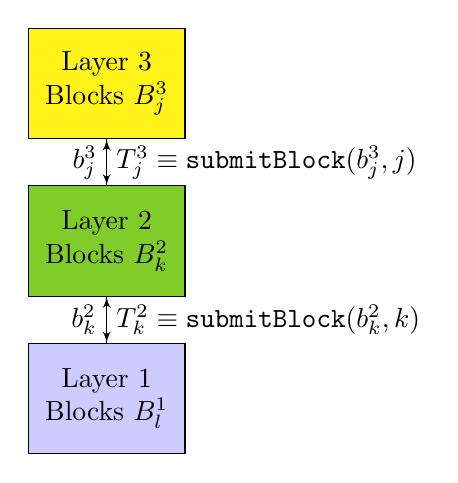
\begin{tikzpicture}[node distance = 2cm, auto]
    % Place nodes
    \node [blockchain3] (l3) {Layer 3 Blocks $\block{3}{j}$};
    \node [blockchain2, below of=l3] (l2) {Layer 2 Blocks $\block{2}{k}$};
    \node [block, below of=l2] (l1) {Layer 1 Blocks  $\block{1}{l}$};
    % Draw edges
    \path [line] (l3) -- node {$\transaction{3}{j} \equiv \submitblock{j}{\blockhash{3}{j}}$} (l2);
    \path [line] (l2) -- node {$\transaction{2}{k} \equiv \submitblock{k}{\blockhash{2}{k}}$} (l1);
    \path [line] (l2) -- node {$\blockhash{3}{j}$} (l3);
    \path [line] (l1) -- node {$\blockhash{2}{k}$} (l2);
\end{tikzpicture} &
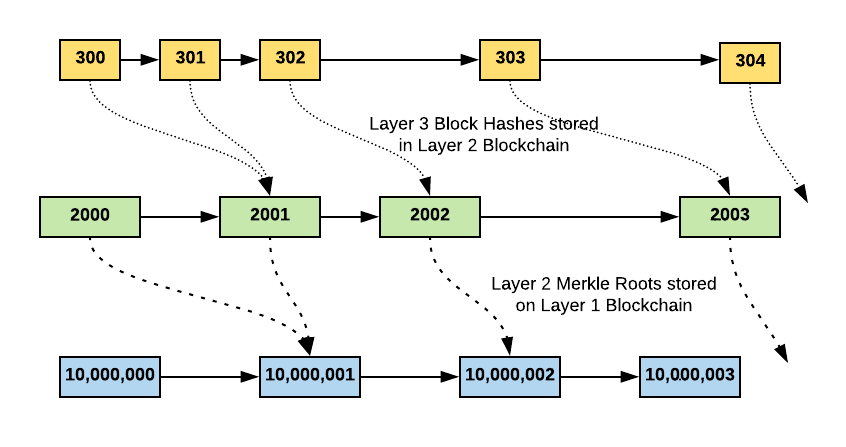
\includegraphics[width=10cm]{Timeline.png} \\
\end{tabular}
}
\caption{Deep Blockchains: In the deep blockchain architecture explored here, each  layer $i+1$ is connected to layer $i$ with transactions submitted to layer $i$ for every block at layer $i+1$. Typically, block hashes and Merkle roots are submitted in transactions as key attributes of the block.}
\centering
\label{timeline}
\end{figure}

Historically, the low-throughput high-latency of Layer 1 blockchains resulted in immediate pressure to drive activities off-chain, but
only a few ``off-chain'' attempts can be considered deep blockchains because they lack the connected blockchains.  Layer $i+1$ and layer $i$  may be explicitly connected in a deep blockchain system for many different reasons:
\begin{enumerate}
    \item Higher throughput services at layer $i+1$ may be paid for using the value held in layer $i$ currency

    \item Storing a limited set of information in layer $i+1$ in layer $i$ may support the security and provenance of layer $i$
    
    \item Proof of fraud at layer $i+1$ can be used for economic consequences at layer $i$
\end{enumerate}
The nascent label ``Layer 2'' encompasses many newly developing notions ranging from state channels to almost any approach that may help Layer 1 scale (e.g. bigger blocks), but we use the term ``deep blockchain'' not for all Layer 2 notions but specifically for any situation where one or more blockchains are {\em connected} in the above way.

\section{Layer 2: Plasma Cash Blockchain}

Seminal insights on multi-layer blockchains were put forth by \cite{poonbuterin2017}, which have inspired many ``Plasma'' designs, and specifically motivated our implementation of what has been termed ``Plasma Cash'' for tracking storage and  bandwidth balances.  The Layer 2 Plasma Cash blockchain is connected to Layer 1 using the following trust primitives:
\begin{itemize}
\item User Deposit: When Alice wishes to use the services enabled by the Layer 2 blockchain, Alice deposits some Layer 1 currency $\lambda_{dep}$ (.01 ETH or 1 WLK) in a Layer 1 contract function (\texttt{createBlockchain}); the deposit event results in Alice owning a Layer 2 token $\tau$ through a Layer 2 Deposit transaction included in a Layer 2 block.

\item User Transfer: When Alice wishes to transfer her Layer 2 token $\tau$ to another user Bob or the Plasma operator Paul, Alice signs a Layer 2 token transfer transaction specifying the recipient and the previous block.  This Layer 2 transaction is included on the Layer 2 blockchain by Paul.   

\item Layer 2 Block Connection: The operators of the Layer 2 blockchain mints new Layer 2 blocks $\block{2}{j}$ with a collation of Layer 2 transactions $\transaction{2}{k}$ (with a consensus protocol such as Quorum RAFT and POA in permissioned networks or Ethereum Casper for permissionless networks) from the User Deposit and User Transfer transactions.  Each Layer 2 block $\block{2}{k}$ has its Merkle Root $\blockhash{2}{k}$ submitted to Layer 1 with a transaction $\transaction{2}{k} = \submitblock{k}{\blockhash{2}{k}}$ recorded in a Layer 1 block $\block{1}{l}$.   The recipient Bob of a token transfer must receive the full history of all transactions from Alice and verify it against these Merkle Roots $\blockhash{2}{k}$ stored in Layer 1, all the way to the original deposit.  If any transaction in the history cannot be verified by Bob, Bob cannot accept Alice's token as payment.  

\item User Exit: When Alice wishes to withdraw her token $\tau$ for Layer 1 cryptocurrency, she calls $\startexit$ function with the last 2 transactions\footnote{As to why {\em two}, two is indicative, but not conclusive concerning Alice's ownership, therefore a user challenge process is required.} which can be verified against and Merkle proofs that must match the stored Merkle roots to be a valid exit; if no one challenges the exit, Alice receives the outstanding token balance within a short time period when exits are finalized.  

\item User Challenges:  If the operator Bob or another user Charlie notices that Alice's exit attempt is invalid, it submits a Merkle proof and rewarded when a valid challenge indicates a invalid exit.
\end{itemize}
Remarkably, users of the Layer 2 blockchain can conduct their business securely even when the Layer 2 operator has 100\% control over the Layer 2 blockchain!  Any sign of malicious operator Paul and the Layer 2 users can exit, and all Layer 2 token values remain secure.  How can practitioners reconcile instincts to pursue this objective:

\begin{center}
   {\bf Blockchain 1.0 Objective:} {\em Maximize decentralization.}
\end{center}

\noindent with an obviously centralized operator?   The answer is to pursue a more nuanced objective of

\begin{center}
   {\bf Blockchain 2.0 Objective:} {\em Maximize the cost of successful attacks.}
\end{center}

With the Plasma Cash construct, the Blockchain 2.0 Objective is achieved with:
\begin{enumerate}
    \item Layer 1 Smart Contracts supporting a Layer 2 Connection to Layer 1 storage that collectively make the cost of attacking the Layer 2 blockchain the same as the cost of attacking the Layer 1 blockchain -- for Ethereum and Bitcoin Layer 1 blockchains, this is the famous ``51\% attack'', for others it might be whatever is required to control the state of that Layer 1 Blockchain.  
    \item Layer 1 Cryptocurrency being used for value transfer of services between users of the Layer 2 Blockchain and the Layer 2 operator mediated through deposits, token transfers and exits mediated by Layer 1 constructs
\end{enumerate}  
With the Layer 2 Block Connection and trust primitives in place, Layer 2 can operate at much higher throughput than Layer 1 because of its reduced consensus, but continuing to inherit Layer 1's cost of attack and achieving the more fundamental objective.  Therefore practitioners of deep blockchain engineering must develop different instincts, incorporating different software trust primitives between different constructed layers to achieve the same objective depending on the structure of between layers and the value unlocked in each.  

\section{Deep Blockchains for Provable Data Storage}

\begin{figure}[t]
\begin{tabular}{c}
\centerline{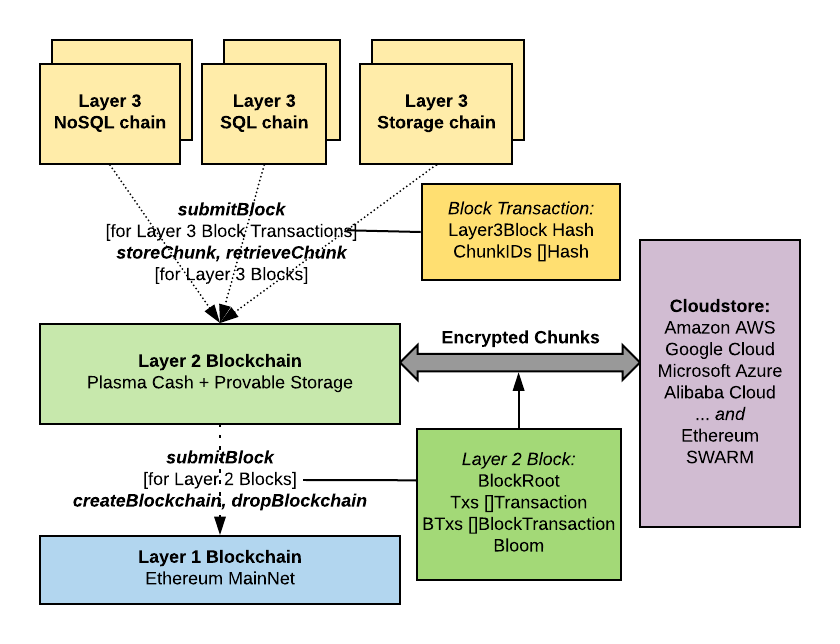
\includegraphics[height=10cm]{Deep-Blockchain.png}}
\end{tabular}
\caption{Deep Blockchain for Storage:  Users of NoSQL/SQL/Storage Layer 3 blocks createBlockchains on Layer 1, and use Layer 2 Plasma Cash to operate their blockchain.  Layer 3 blocks are submitted to the Layer 2 Blockchain via anchor transactions and chunks are insured.  Plasma Tokens are used for bandwidth.  Cloudstore combines major computing platforms with Ethereum SWARM for both resilience and speed.}
\centering
\label{deepblockchain}
\end{figure}

The specific deep blockchain system that we have developed extends the Blockchain 2.0 Objective up one more layer by incorporating trust primitives (Anchor transactions, Sparse Merkle Trees) in provable NoSQL, SQL and Storage services, shown in Figure 2:  Layer 3 NoSQL, SQL and Storage blockchains rest on the storage and bandwidth services of Layer 2, which supervene on the decentralized computation and payment services of Layer 1.  Our work follows Ethereum SWARM's foundational work on storage and bandwidth \cite{swarm} which outlines the following ideas that we situate in multiple layers:
\begin{itemize}
    \item A chunk of bytes $v$ is stored in Cloudstore using 256-bit hash $k = \hash{v}$ as the key to retrieve $v$.  Nodes that request a chunk by key $k$ can verify correctness of the value $v$ returned from Cloudstore simply by checking if   $k=\hash{v}$. 
    \item Insurers of chunks can earn Layer 1 currency with valid Merkle proofs; Failure to provide valid proofs result in severe insurance payouts
    \item Bandwidth consumed by a node, when hitting the nodes threshold must result in signed payments 
\end{itemize}
Layer 1 blockchains were initially developed without the concern for storage models being competitive with cloud computing platforms or even a passing concern for bandwidth; the birth of Bitcoin and Ethereum Layer 1 focused on birthing trustless payments and trustless computation mediated by a peer-to-peer network, rather than about nodes providing decentralized storage.   In contrast, decentralized {\em storage} networks, as manifested in Ethereum SWARM and many other systems, promises to have a large peer-to-peer network of nodes sharing the responsibility to keep a portion of the world's data and compensated proportionately for the commodity storage and bandwidth they provide.  In these networks, a distributed hash table (typically, with Kademlia routing layers) is used for logarithmic look ups of chunks, but in practice, $O(log_2(n))$ retrieval times are just not competitive with modern UI expectations or typical developer expectations.  Nevertheless, decentralized storage networks have a critical role to play in providing censorship-resistance.  Rather than layer 3 rest solely on a decentralized storage network (which is slow but resilient and censorship-resistant), we can rest layer 3 on {\em both} decentralized storage networks {\em and} mature modern cloud computing platforms.  Again, the Blockchain 1.0 Objective must be displaced in favor of the Blockchain 2.0 Objective: in this sense, more storage variety {\em increases} the cost of attack.  

Putting the elements together in a deep blockchain system for provable storage: 
\begin{itemize}
\item Layer 1 blockchain: When a developer wishes to have a Layer 3 blockchain for NoSQL/SQL/Storage, they send Layer 1 currency into \texttt{createBlockchain(blockchainName string)} on MainNet; this can be refunded with a {\tt dropBlockchain(blockchainName string)} operation (taking place of {\tt startExit}).  When storage is used in {\tt blockchainName} through the activities of Layer 3 blockchains (as recorded by the Layer 2 blockchain below), this balance goes down.  Balances can added to and withdrawn by the owner of the blockchain.

\item Layer 2 Plasma Cash Blockchain: The storage and retrieval of chunks in Cloudstore are exposed to Layer 3 blockchains with the following 2 APIs (see Appendix A):
\begin{itemize}
    \item \texttt{storeChunk}$(k, v, \tau, \signature)$ - stores a key-value pair mapping $(k,v)$ in Cloudstore, backed by Layer 2 token $\tau$ (signed with $\signature$) received from the Layer 1 transaction.  
    \item \texttt{retrieveChunk}$(k, \tau, \signature)$ - retrieves a key-value pair mapping $(k,v)$ in Cloudstore, backed by Layer 2 token $\tau$ (again, signed with $\signature$), and returning the balance of $\tau$ used so far  
\end{itemize}
The Layer 2 operator will store via Cloudstore in as many regions and cloud providers as necessary to {\bf insure} the chunk as follows:  A new type of Layer 2 {\bf anchor transaction} insures a set of chunks recorded through \texttt{storeChunk} calls.  The cause of these chunks are from any Layer 3 blockchain needing storage and bandwidth, where bandwidth is used in \texttt{retrieveChunk} calls.  When a Layer 3 blockchain mints Layer 3 blocks, the Layer 3 blocks themselves contain a Cloudstore key that references a list of chunks written in the Layer 3 block.  The block itself is stored in Cloudstore with another \texttt{storeChunk} call, signed by the Layer 3 blockchain owner, and the block hash $\blockhash{3}{k}$ is submitted by the Layer 3 blockchain to the Layer 2 blockchain via a $\submitblock{k}{\blockhash{3}{k}}$ anchor transaction.  This enables the Layer 2 blockchain to meter the cumulative storage of {\tt blockchainName} and deduct from the balance originally deposited in the $\texttt{createBlockchain(blockchainName string)}$ operation (approximately every 24 hours), passing on Cloudstore costs to Layer 3 blockchains.  Notably, Layer 3 blocks themselves are recorded with $\texttt{storeChunk}(k, v, \tau, \signature)$ to store the layer 3 block in Cloudstore and then results in a call to $\submitblock{j}{\blockhash{3}{j}}$:
\begin{equation}
\transaction{3}{j} \equiv \submitblock{j}{\blockhash{3}{j}}
\end{equation}
Because both the block storage and anchor transactions are signed, Layer 2 operators collect storage payments with the layer 3 blockchain operator's consent, forming a kind of ``state channel'' within the deep blockchain.  Taken together, this is the Layer 3 Block Connection, as seen in Figure \ref{timeline}.  The Layer 2 block consists of:
\begin{itemize}
\item the transaction root $\transactionroot{2}{k}$ that utilizes the SMT structure to represent just the tokens $\tau_1, \tau_2, \ldots$ spent in block $k$
\begin{equation}
\transactionroot{2}{k} \equiv \texttt{KT}( (\tau_1, \transaction{2}{\tau_1}), (\tau_2, \transaction{2}{\tau_2}), ... )
\end{equation}
\item the token root $\tokenroot{k}$  for {\em all} tokens $\tau_j, ...$
\begin{equation}
\tokenroot{k} \equiv \texttt{KT}( (\tau_1, \transaction{2}{\tau_1}), (\tau_2, \transaction{2}{\tau_2}), ... ) 
\end{equation}
\item array of token transactions  $\transaction{2}{k}$
\item array of anchor transactions  $\anchortransaction{2}{k}$ from all Layer 3 blockchain operators using Layer 2 services 
\item an account root, using an SMT to store an accounts ``balance'' and a list of tokens held by that account.
\end{itemize}

\item Layer 3 blockchains:  Any number of Layer 3 blockchains that utilize storage and bandwidth can be layered on top of the Layer 2 blockchain, regularly submitting lists of chunks based on the structure of the Layer 3 blockchain.  
\begin{itemize}
    \item For NoSQL + File Storage, there is a key for each row of NoSQL or File, and a value for the row (a JSON record) or raw file contents.   The root hash changes when any table is added/removed or when any table schema is updated, and where each table has a root hash that changes when any record of the table is changed; any new database content results in new chunks, where the chunk is referenced by the hash of its content.
    \item For SQL, there is a root hash for each database, where the root hash changes when any table schema is updated, and where each table has a root hash that changes when any record of the table is changed; any new database content results in new chunks, where the chunk is referenced by the hash of its content.
\end{itemize}  
We describe both NoSQL and SQL Blockchains in Section ~\ref{sec:layer3}.
\end{itemize}

\noindent Just as with Layer 1 blockchain nodes, running Layer 2 and Layer 3 blockchains consists of running a node in a peer-to-peer network, receiving and transmitting messages about new transactions and new blocks.   Wolk's blockchain implementations of the Layer 2 and Layer 3 originated from Ethereum's \href{https://github.com/ethereum/go-ethereum}{go-ethereum} and JPMorgan's \href{https://github.com/jpmorganchase/quorum}{Quorum RAFT} code bases, written in Golang.  We used RAFT for both Layer 2 and Layer 3 implementations due to its simple model of finality.  For each blockchain, we created a Golang package containing each of the interfaces specified in Appendix A, and adapted Quorum RAFT code to conform to these interfaces.  There is no explicit assumption that  permissioned consensus algorithms be used, however.   The choice of RAFT was made purely out of simplicity, its maturity as a code base, and its capacity for high throughput -- any consensus protocol that achieves finality can fit within this deep blockchain architecture.  For both the Layer 2 and Layer 3 blockchains, we use a \href{https://github.com/wolkdb/deepblockchains/smt}{Sparse Merkle Tree} to support provable data storage, which we review in detail next.

\section{Sparse Merkle Trees and Provenance}

The Sparse Merkle Tree (SMT) is a persistent data structure that map fixed $q$-bit keys to 256-bit values in an abstract tree of height $q$ with $2^{q}$ leaves for any set $\mathfrak{I}$:
\begin{equation}
\mathfrak{I} = \{ (\mathbf{k}_0 \in \mathbb{B}_{q}, \mathbf{v}_0 \in \mathbb{B}_{256}), (\mathbf{k}_1 \in \mathbb{B}_{q}, \mathbf{v}_1 \in \mathbb{B}_{256}), \ldots \}
\end{equation}
The function of the SMT is to provide a unique Merkle root hash that uniquely identifies a given set of key-value pairs $\mathfrak{I}$, a set containing pairs of byte sequences.  Each key stored in the SMT defines a Merkle branch down to one of $2^{q}$  leaves, and the leaf holds only one possible value for that key in $\mathfrak{I}$. The bits of the $q$-bit key define the path to be traversed, with the most significant bit at height $q-1$ and least significant bit at height $0$.  Following \cite{lauriekasper2012} and \cite{Dahlberg2016EfficientSM}, to compute the Merkle root of any SMT in practice, just the Merkle branches for the $n$ Merkle branches need to be computed, and to do this efficiently it is useful pre-compute a set of default hashes $\defh{h}$ for all heights h from $0 \ldots q-1$ levels: (shown in Figure~\ref{smt})
\begin{itemize}
\item At level 0, $\defh{0} \equiv \hash{0}$
\item At level $h$, $\defh{h} \equiv \hash{ \defh{h-1}, \defh{h-1} }$
\end{itemize}
Logarithmic insertion, deletion and retrieval operations on the SMT are defined with elemental operations:
\begin{itemize}
    \item \texttt{insert}$(k,v)$ - inserts the key by traversing chunks using the bytes of $k$
    \item \texttt{delete}$(k)$ - deletes the key by inserting the null value for $k$ into the SMT
    \item \texttt{get}$(k)$ - gets the value from the SMT through node / chunk traversal
\end{itemize}
Typically, block proposals with SMTs as a core data structure involve bulk combinations of the above, with many inserts and deletes mutating the content of many chunks, and the Merkle root only being computed as a final step.

Sparse Merkle Trees are best suited for a core primitive over more familiar Binary Merkle Trees (BMTs) because:
\begin{itemize}
\item when an id (a tokenID, a document key in NoSQL, a URL in File storage, a table root in SQL) is mapped to a value, you can guarantee that the id has exactly one position in the tree, which you don't get with BMTs.
\item when an id is NOT present in the SMT, you can also prove it with the same mechanism. This will come in handy when Bloom filters generate false positives.
\item   A Merkle proof for the id mapped to a specific value is straightforward, and because of sparseness the number of bytes required is much less than the depth of the tree
\end{itemize}
The central idea behind SMTs representing which ids have been included in the SMT is you can keep $n$ hashes of the $n$ ids used at just $n$ of the $2^q$ leaves, where each id is a $q$-bit number; because $n << 2^q$, and with ids made truly sparse with a hash function (e.g Keccak256), there is either a ``null'' or the hash of the value at each leaf.  A typical Merkle proof for a 64-bit id is {\em not} 64 32-byte hashes going all the way from level 0 at the leaf all the way to the root! Instead, $q$ bits of $\proofBits$ (with $q=64$, \texttt{uint64}) can compactly represent whether the sisters going up to the root are default hashes or not - that is, for each bit, $0$ means ``use the default hash'', and  1 means ``use 32 bytes in $\proofBytes$'' -- where the $\proofBytes$ contains {\em just} the non-default hashes. At the leaf of the Merkle branch it is natural to keep the 32-byte RLP hash of the value being stored.

\begin{figure}[t]
\begin{tabular}{c}
\centerline{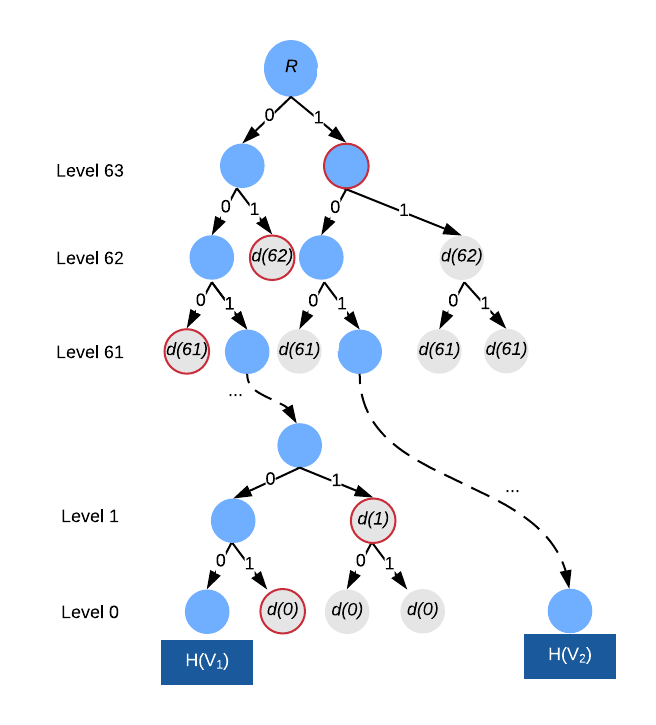
\includegraphics[width=8cm]{SMT.png}} \\
\end{tabular}
\caption{\small Sparse Merkle Tree Illustration: Merkle branches for 2 64-bit keys $k_1=\texttt{001..00}$ and $k_2=\texttt{101..}$ hold $\hash{V_1}$ and $\hash{V_2}$ in a unique SMT root $R$ for a 2 key set $\mathfrak{I} = \{ (K_1, V_1), (K_2, V_2) \}$. Since there are only keys in this tree, the default hashes $d(h)$ (outlined in red) appear starting at level 62, so the branches $K_1, K_2$ (shown in blue circles) have Sparse Merkle proofs using default hashes from level 0 to level 62, which can be specified in a \texttt{proofBits} parameter.  This makes for very tiny proofs and lower gas costs on MainNet. }
\centering
\label{smt}
\end{figure}

For the Layer 2 Block Connection, a call to 
\[
\texttt{checkMembership(bytes32 leaf, bytes32 root, uint64 tokenID, uint64 proofBits, bytes proofBytes)}
\]
helper function in Ethereum MainNet can take $\proofBits$ and $\proofBytes$ and prove that a exit or challenge is valid if it matches the Merkle roots provided by the Plasma operator in a call to 
\[
\texttt{submitBlock(bytes32 root)}
\]
Likewise, one user receiving a token from another user must (without any checkpoint finalization concepts) get \texttt{tokenID}, along with $t$ raw txbytes, and $t$ Merkle proofs, where each Merkle proof concerns the spend in a specific block. But note that a non-spend also can be proven as well, where the leaf is $H(0)$. 

In the best case, a single id in an SMT represents the just one key-value mapping ($n=1$), and instead of a $64 \times 32$ byte proof, you have default hashes all the way from level 0 to level 63, and $\proofBits$ is 64 zeros (\texttt{0x0000000000000000}). You have $\proofBytes$ being nothing and a $\texttt{uint64}$ being $\texttt{0}$, which is as compact as it gets! Proof size: 8 bytes.

In the next best case, with 2 ids (say, \texttt{0x01234...} and \texttt{0x89abc...}) the proof of spend of each token would have one non-default hash up at top in level 63 and \texttt{proofBits} being 1 followed by 63 zeros (\texttt{0x8000000000000000}). Proof size: 40 bytes.

For non-contrived cases, SMTs will have very dense upper nodes from level $q-1$ down to around level $log_2(n)$. To make this concrete, lets say you have 10MM Layer 2 tokens, where each token undergoes 500 transactions per token per year. Then you'll have 5B transactions for your 10MM tokens each year. If your Layer 2 block frequency is 15s/block, then you'll have these 5B transactions distributed over 2.1MM blocks/yr, with an average of 2,378 transactions per Layer 2 block ($500 \times 10 \times \frac{10^{6}}{86400 \times \frac{365}{15}}$). When you put these 2,378 transactions into an SMT, because $log_2(2378)=11.2$, you'll have a super dense set of nodes mostly having non-default hashes for levels 63 down to level 53 or so, and then below that you will have just one tokenID going all the way down to level 0. Proof size: 32 bytes $\times$ 10 levels, or 320 bytes.

We decided on $q=64$ instead of $q=256$ because: 
\begin{itemize}
\item collisions are still unlikely at q=64 ... until you get around 4B keys
\item the $\proofBits$ are 24 bytes smaller (\texttt{uint64} instead of \texttt{uint256})
\item less gas is spent in \texttt{checkMembership} on all 0 bits in $\proofBits$
\item we can have a smaller 64-element array of default hashes computed instead of 256 hashes
\end{itemize} 
Less hashing means less gas and happier users, at least at the Level 2 block connection, where collisions between circulating tokenIds can be verified to be impossible on deposit events.  Moreover, you can combine the fixed length $\proofBits$ and variable length $\proofBytes$ into a single proof bytes input for exits, i.e. \texttt{startExit(uint64 tokenID, bytes txBytes1, bytes txBytes2, bytes proof1, bytes proof2, int blk1, int blk2)}  The analogous challenge interfaces will then have fewer argument inputs in the same way.

The sparseness of the SMT derives from the observation that keys will extremely rarely share paths at increasingly lower heights and naturally will share paths at increasingly higher paths.  This lends itself to a representation where the SMT is chunked by byte $\mathbf{k}_i$, where traversing the SMT from a root chunk (representing a range of keys from 0 to $2^{64}$-1) down to an intermediate chunk with just one leaf involves processing one additional byte, which each chunk of data storage having up to 256 child chunks specifying a range of keys each child posessing a range that is $\frac{1}{256}$ smaller.  Just as with a radix tree, the SMT is traversed from root to leaf, with an additional byte of the key causing a read of a chunk that represents up to 256 branches and the hashes of all the branches, utilizing default hashes.  We implemented a Golang "smt" package and a "cloud" package to map SMT operations into Cloudstore.

\section{Layer 3 Blockchains\label{sec:layer3}}

With the foundations of Layer 2 providing storage and bandwidth, paid for with Layer 2 tokens, any number of Layer 3 blockchains may be constructed.  We detail the construction of a NoSQL and SQL blockchain here.  At a high level, Layer 3 blockchains collate SQL and NoSQL transactions in Layer 3 blocks and submit anchor transactions to Layer 2. On the Layer 2 blockchain, token and anchor transactions are collated with Merkle Roots of token root and blocks submitted.  These are then submitted from the Layer 2 blockchain as anchor transactions to the Layer 1 blockchain.  It then becomes possible to aggregate multiple proof of inclusions at the highest layers all the way to MainNet with Deep Merkle Proofs, which we illustrate here.

\subsection{Layer 3 NoSQL Blockchain and Deep Merkle Proofs}

To support Layer 3 NoSQL transactions in a NoSQL blockchain, the Layer 3 blockchain has a layer 3 block structure defined as collating a set of NoSQL records along with a {\tt Layer3KeyRoot} of a Sparse Merkle Tree managing a set of key-value pairs of ``documents''.  All NoSQL records are encrypted using counter mode (CTR) encryption defining operations $\encrypt{d}$ and $\decrypt{d}$ and utilizing a database encryption key $\databaseencryptionkey$ known only to the layer 3 blockchain user.   Three operations are defined, each of which map into the SMT data structure: 
\begin{itemize}
\item \texttt{SetKey}$(k,v)$ - stores arbitrary $k,v$, through a \texttt{storeChunk}(k, v) Layer 2 operation and a Layer 3 SMT operation on $\keyroot$ (\texttt{insert}($\hash{k},\hash{\encrypt{v}}$)) 
\item \texttt{GetKey}$(k)$ - retrieves the value $v$ stored in the {\tt SetKey}$(k,v)$ operation, through Layer 3 operation on $\keyroot$ \texttt{get}(\hash{k}) which returns $v_h$ followed by $\decrypt{\texttt{retrieveChunk}(v_h)}$ 
\item \texttt{DeleteKey}$(k)$ - removes $k$ from the NoSQL database, by storing $(\hash{k},\emptyhash)$ in the SMT; subsequent calls to \texttt{GetKey}(k) will not return a value.
\end{itemize}
The minting of a new Layer 3 NoSQL Block consists of taking each of the Layer 3 transactions ($\texttt{SetKey}, \texttt{DeleteKey}$), executing  \texttt{storeChunk} Layer 2 API calls for its users.  Unless two transactions operate over the same key $k$, all transactions can be executed in parallel.  If multiple transactions operate over the same key, only the last received transaction will have its mutation succeed.  

We present a detailed example: (shown in Figure~\ref{deepmerkleproof})
\begin{itemize}
\item In Layer 3 Block 302, the user wishes store document ID 1 with key $K_1$ mapped to encrypted value $V_1$ and document ID 2 mapped to encrypted value $V_2$. The user can submit 2 Layer 3 NoSQL transactions: 
\begin{equation*}
\left[ \texttt{SetKey}(K_1=\texttt{0b001...00},V_1=\texttt{0x778899..}), 
\texttt{SetKey}(K_2, V_2)
\right]
\end{equation*}
\noindent which results in a set of SMT primitive operations: 
\begin{equation*}
\{\texttt{insert}(\hash{K_1},\hash{\encrypt{V_1}}),  \texttt{insert}(\hash{K_2},\hash{\encrypt{V_2}}) \}
\end{equation*}
resulting in 
$\texttt{Layer3KeyRoot}=\texttt{0x83fc...}$.  The chunks for both documents $H(V_1)$ and $H(V_2)$ along with chunk of the previous block 301  (e.b. \texttt{storeChunk(0b001.., ...)}) are included in Layer 3 Block 302 in the \texttt{ChunkIDs} and insured with a call to \[
\texttt{submitBlock(0b101..11, 302}
\]
submitted to the Layer 2 blockchain. 

\item When the Layer 2 blockchain processes the anchor transactions from this new Layer 3 block (and many other Layer 3 blockchains) to build Layer 2 Block 2002, it will build a SMT with 
\[
\texttt{insert(concat(blockchainName, 302), 0b001..00)}
\]
(and other inserts) to generate a \texttt{BlockRoot} (e.g. \texttt{0x4d69..}).  As is standard, the new \texttt{BlockRoot} uses the previous block's \texttt{BlockRoot} as a starting point.  Packaging the anchor transactions together with any token transactions (balance updates, transfers, deposits, etc.), the new layer 2 block 2002 with hash \texttt{0xe8db..} will be stored in Cloudstore with a call to $\texttt{storeChunk(0xe8db...)}$ 
Txs and submitted to Layer 1 with a call to 
\[
\texttt{submitBlock(0xe8db..., 2002)}.  
\]
\item Finally, a Layer 1 Block (e.g. 10,000,002) will be proposed by some MainNet miner including the above Layer 2 $\texttt{submitBlock}$ transaction and eventually be finalized by the Layer 1 consensus protocol.
\end{itemize}

\begin{figure}[t]
\begin{tabular}{c}
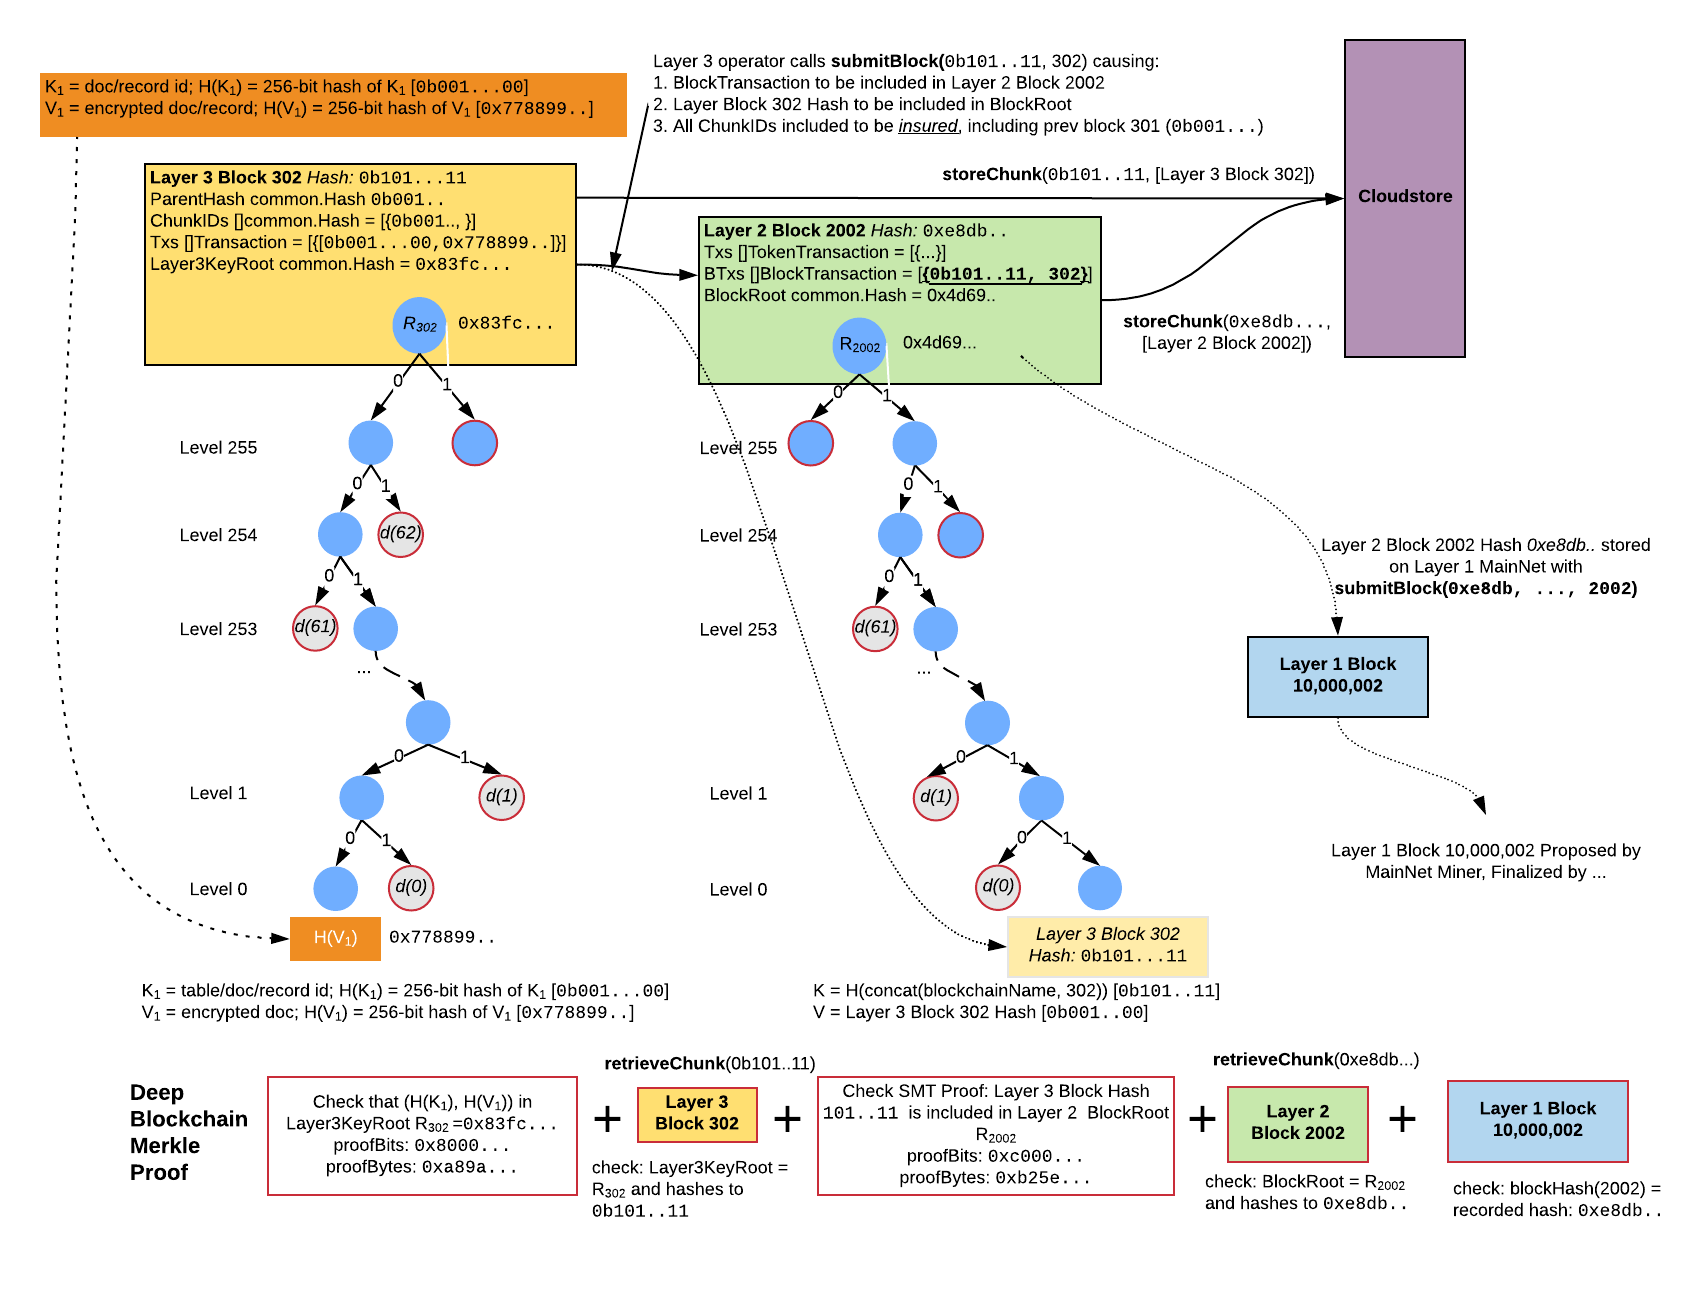
\includegraphics[width=17cm]{DeepMerkleProof.png} \\
\end{tabular}
\caption{\small Deep Merkle Proof illustrated: The hashes key-value pair is recorded in a Layer 3 Sparse Merkle Tree, the root of which is kept in \texttt{Layer3KeyRoot} in the Layer 3 block.  When the Layer 3 operator uses \texttt{submitBlock} to submit a {\em anchor transaction} to Layer 2,  Layer 3 Block hash 302 is included in another SMT maintained by the Layer 2 operator storing all Block hashes of all Layer 3 blockchains.  When the Layer 2 block 2002 is minted, the \texttt{BlockRoot} is set and included in Layer 1 Block 10,000,002.  The individual proof of inclusion from the 2 SMTs and the portions of the raw Layer 3 and Layer 2 block form a {\em Deep Merkle Proof} for inclusion a specific record in the deep blockchain, from the highest layer to Layer 1.}
\centering
\label{deepmerkleproof}
\end{figure}

A Deep Merkle Proof is formed through the aggregation of each proof of inclusion across each layer of blockchain connections in a deep blockchain down to Layer 1.  In our 3 layer deep blockchain with the Layer 3 NoSQL blockchain layered on the Layer 2 Storage / Plasma Cash blockchain, there is a Layer 2-3 connection and a Layer 1-2 connection.  So a full Deep Merkle Proof that a NoSQL document $K_1, V_1$ is included in the deep blockchain all the way up to MainNet consists of: 
\begin{enumerate}
\item Layer 3 proof of inclusion of $(H(K_1), H(V_1))$ in Layer 3 block $\texttt{Layer3KeyRoot}$ -- in our example, this would be that the value $\hash{V_1}$ hashes up to SMT root $R_{302}=\texttt{0x83fc..}$.

\item Layer 2 proof of inclusion of $(\hash{\texttt{concat(blockchainName, k)}})$ in Layer 3 block $\texttt{Layer3KeyRoot}$ -- in our example, this would be that the Layer 3 block hash  $\texttt{0b101..11}$ hashes up to SMT root  
 $R_{2002}=\texttt{0x4d69..}$    
 
\item Layer 1 proof of inclusion of the Layer 2 block hash in the \texttt{blockHash} array of the Layer 1 Smart Contract -- in our example, this is that \texttt{blockHash(2002) = 0xe8db}  
\end{enumerate}
In our implementation, deep Merkle proofs are provided in response to $\texttt{GetKey}(K,V)$ to the layer 3 blockchain users as an optional \texttt{deep} boolean parameter and when true,  returns the full combination of:
\begin{itemize}
    \item Layer 3 Block, which includes $\texttt{Layer3KeyRoot}$
    \item $\proofBits$ and $\proofBytes$ for the Layer3KeyRoot, which are shown to match $H(K), H(V)$
    \item Layer 2 Block, which includes $\texttt{BlockRoot}$
    \item $\proofBits$ and $\proofBytes$ for the $\texttt{BlockRoot}$, which are shown to match the Layer 2 Block Hash
    \item Layer 1 blockHash record of the Layer 2 block number    
\end{itemize}

The concept of a deep Merkle Proof is not limited to 3 layer deep blockchains, nor is the concept only applicable to NoSQL blockchains -- the concept applies to multiple layers of proof of inclusion enabled through the general layering processes of deep blockchain systems generally.

\subsection{Layer 3 SQL Blockchain}

To support Layer 3 SQL operations in a SQL blockchain, the Layer 3 block has a  structure defined as having as packing a set of encrypted SQL transactions ({\tt insert}/{\tt update}/{\tt delete} statements)  along with a $\texttt{Layer3KeyRoot}$ of a Sparse Merkle Tree representing a set of table root hashes.

In our implementation, we adapted Quorum RAFT as the consensus layer for our layer 3 SQL blockchain (again, following Appendix A), which collectively follow a consensus protocol where once a {\em leader} has been identified, the leader mints a new Layer 3 block based on: 
\begin{itemize}
\item An array of SQL transactions that is mapped into newly created chunks (created via $\texttt{storeChunk}$ for table root hashes)
\item An array of table root hashes, key-value pairs written to $\texttt{Layer3KeyRoot}$, based on the execution of the above SQL Transactions 
\end{itemize}  
The minting a layer 3 block consists of the leader compiling each SQL transaction into a set of instructions to executed by a ``SQL Virtual Machine'' (SVM) based off of the widely used SQLite's virtual machine.  In this model, a virtual machine has a program counter that increments or jumps to another line after the execution of each opcode instruction.  For example, a SQL statement of "Select * from person" received by a node is mapped into a interpretable set of opcodes like this:
\begin{verbatim}
{"n":0,"opcode":"Init","p2":8,"p4":"select * from person"}
{"n":1,"opcode":"OpenRead","p2":2,"p4":"2"}
{"n":2,"opcode":"Rewind","p2":7}
{"n":3,"opcode":"Column","p3":1}
{"n":4,"opcode":"Column","p2":1,"p3":2}
{"n":5,"opcode":"ResultRow","p1":1,"p2":2}
{"n":6,"opcode":"Next","p2":3,"p5":1}
{"n":7,"opcode":"Halt"}
{"n":8,"opcode":"Transaction","p3":3,"p4":"0","p5":1}
{"n":9,"opcode":"Goto","p2":1}
\end{verbatim} 
In our SVM Golang implementation, all opcodes are mapped into Layer 2 $\texttt{storeChunk}$ and  $\texttt{receiveChunk}$ calls, manipulating the following chunk types:
\begin{itemize}
\item Database Schema chunk: represents up to 32 tables belonging to the ``blockchainName''.  Each table is identified by name (up to 32 bytes) and has a {\em table chunk};
\item Table chunk: represents up to 32 columns belonging to a specific ``table''.  Each column is identified by name (up to 27-bytes) and additional information: its column type (integer, string, float, etc.), whether it is a primary key, and any index information; a 32-byte chunk ID points to a potential {\em index chunk}, if the column is indexed
A table must have at least one primary key.
\item Index chunk:  a B+ tree, composed of intermediate ``X'' chunks and data ``D'' chunks. Each X chunk has 32-byte pointers to additional X chunks or D chunks. D chunks form a ordered doubly linked list, and contain pointers to {\em record chunks}.
\item Record chunk: a 4K chunk of data that holds a JSON record for a keyed value.
\end{itemize}
Our current implementation has a full implementation of single table operations thus far, but with relational database operations approachable with the same dynamics:
\begin{itemize}
\item When the owner of a Layer 3 blockchain creates a new database, the owner chunk is updated and  database chunk is created and the owner chunk is updated with the new database chunk information. If this is the first database created by the owner, the root hash of the owner is set for the first time. The root hash of the database is set for the first time.
\item When the owner of a Layer 3 blockchain creates a new table, the database chunk is updated and table chunk is created and the database chunk is updated with the new table information.  This also causes the owner chunk to be updated with the new database chunk information.  The root hash of the table is set for the first time in the child chain.
\item When the owner of a Layer 3 blockchain creates or updates a table, this creates or changes the database schema chunk.  The database chunk is then updated with the new schema information, which in turn causes the owner chunk to be updated with the new database chunk information. 
\item When an owner creates a new record in a table with a SQL statement such as
\[
\sql{insert into account (id, v) values (42, "minnie@ethmail.com")}
\]
the index chunks (X chunks and D chunks) are updated with new primary key information and a record chunk is created in JSON form 
\[
\json{{"id":42, "v":"minnie@ethmail.com"}}
\]
Because the index chunk changes, the table chunk changes. The root hash of the table is set for the first time in the child chain.
When an owner updates a record in a table with a SQL statement lie
\[
\sql{update account set v = "minnie@mail.eth" where id = 42}
\]
the record has a new chunkID because of the new JSON content
\[
\json{{"id":42, "v": "minnie@mail.eth"}}
\]
and so one or more index chunks are updated with a new chunkID.
\item When an owner drops a database, the owner chunk is updated globally.  Additionally, any tables associated with the database at the time of deletion should have their root hashes updated.
\item When an owner deletes a table, the root hash of the table is updated, the schema chunk is updated, and the database chunk is updated with the new schema chunk info and removing the table name.  The owner chunk is then updated with the new database chunk info..
\end{itemize}
When the leader node of a Layer 3 SQL blockchain mints a Layer 3 block, it must include in its Layer 3 block:
\begin{itemize}
\item the SQL transactions -- where for each table referenced in the SQL, the leader must retrieve the previous root hash of the table in the SMT and execute the SVM operations for that table against that SMT's data.   

\item the Chunks newly written through the execution of the SQL transactions, where chunks are only created, and never ``updated''.   

\item a  new $\texttt{Layer3KeyRoot}$  transactions and calls $\submitblock{k}{\blockhash{3}{k}}$: for all tables updated from the SQL transactions, each table has a new root hash. 
Using the $\texttt{Layer3KeyRoot}$, any layer 3 node can respond to a SQL \sql{SELECT} query by retrieving the the previous hash of any table from the SMT.
Using the $\texttt{Layer3KeyRoot}$, any layer 3 node can respond to a SQL \sql{SELECT} query by retrieving the the previous hash of any table from the SMT 

\end{itemize}
With a newly minted Layer 3 block $k$, the Layer 3 SQL blockchain can submit an anchor transaction $\transaction{3}{k}$ to the layer 2 blockchain to be included in the Layer 3 Block $\blockhash{3}{k}$
\[
\submitblock{k}{\blockhash{3}{k}}
\]
which proceeds just as in the NoSQL blockchain, with the analogously structured Deep Merkle Proof.  Where in the NoSQL chain, each NoSQL document / row updated resulted in an updated leaf in the SMT for the newly updated document, now with the SQL chain, each SQL statement supports a new table root hash change in an update leaf in the SMT.  
 

\begin{figure}
\begin{tabular}{c}
\centerline{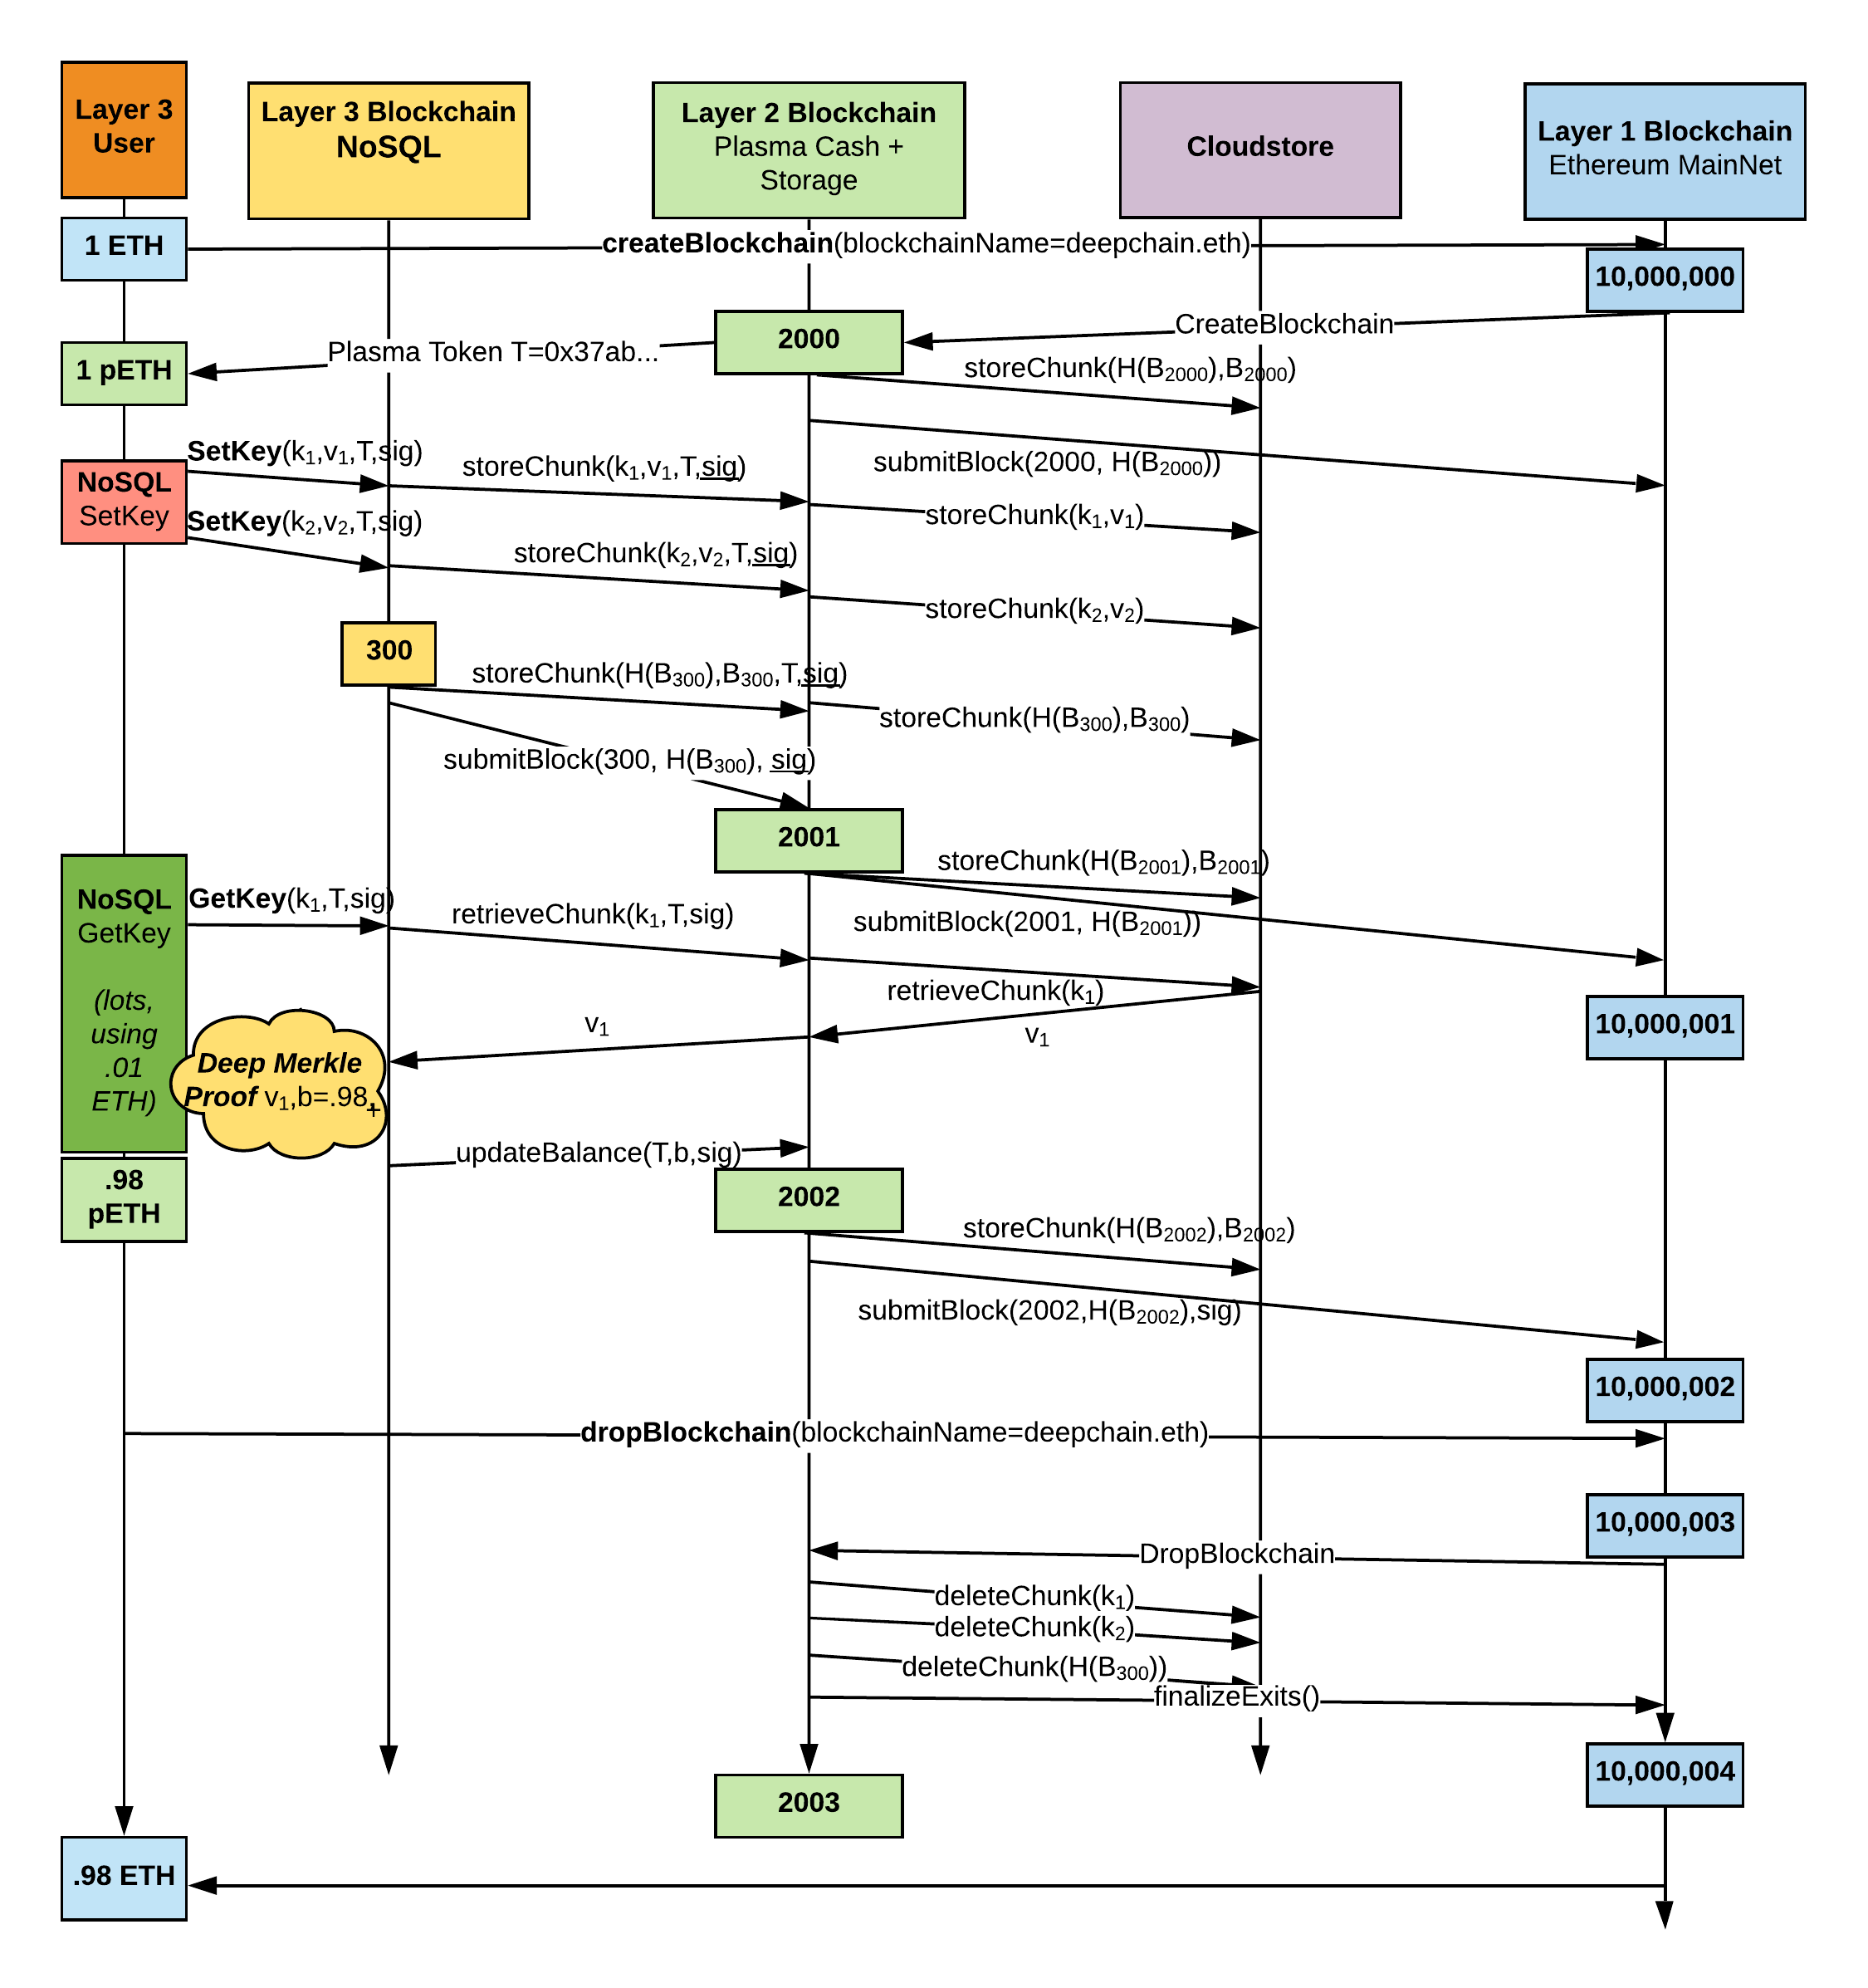
\includegraphics[width=17.5cm]{StateChannel.png}} \\
\end{tabular}
\caption{\small Samples of a Layer 3 NoSQL Blockchain User in the Deep Blockchain architecture presented here.  A Layer 3 user creates a Layer 3 Blockchain by sending 1 ETH to createBlockchain and receives a Plasma token (1 pETH) which is included as a deposit in Layer 2 block 2000.  The Layer 3 user performs 2 SetKey operations included in Layer 3 block 300, which result in the Layer 3 blockchain signing 2 \texttt{storeChunk} for each key-value pair.  The Layer 3 blockchain mints Layer 3 Block 300 and stores it again with 3rd signed \texttt{storeChunk} call, finally calling Layer 2's \texttt{submitBlock} with the hash of Block 300.  The Layer 2 operator includes this anchor transaction in Layer 2 Block 2001, stores it in Cloudstore, and submits it the Layer 1 blockchain with a Smart Contract call to \texttt{submitBlock}.  Later, multiple (lots and lots)  of signed  \texttt{GetKey} calls are done by the Layer 3 User, each executed using \texttt{retrieveChunk} signed calls.  At some point, the user hits $\Sigma_{max}=.02 pETH$ and uses \texttt{updateBalance} to agree that its balance is 0.98 pETH, which is included in Layer 2's token transaction block and submitted to Layer 1.  Finally, the Layer 3 user can drop its blockchain, which will trigger deletion of chunks and initiate a finalizeExit process that returns the .98 ETH balance to the user.}
\centering
\label{statechannel}
\end{figure}

\section{Paying for Storage and Bandwidth}
The Layer 3 blockchain users who store NoSQL/SQL/File data with
\texttt{storeChunk} operations give the Layer 2 operator permission to charge for bandwidth and storage in two different ways:

\begin{enumerate}
\item {\em Bandwidth} is paid for through (1) users signing  \texttt{retrieveChunk}$(k, \tau, \signature)$ calls to retrieve data and obtain recent balances, where each call uses up a tiny amount of bandwidth backed for with a token $\tau$ originated by the \texttt{createBlockchain} call; (2) users signing a new \texttt{updateBalance} request originated by operator agreeing to latest balances. An updateBalance response by the user is mapped to layer2 transactions, where incurred bandwidth cost is deducted from token $\tau$'s owner balance and added to operator's allowance.

\item {\em Storage} is paid for through Anchor Transactions $\submitblock{k}{\blockhash{3}{k}}$ signed by the Layer 3 blockchain operator - because chunks are identified directly inside Layer 3 blocks, a tally of the number of bytes used in each new layer 3 block is added to the SMT.  The Layer 1 contract then exposes \texttt{storageCharge} interface to the Layer 2 operator where a recently signed Layer 2 anchor transaction (containing a tally of the number of bytes, signed by the Layer 3 blockchain operator) is used to deduct the layer 3 operator's balance since the last time it was called.   This is detailed below.
\end{enumerate}
In this way Layer 3 Blockchains pay for the services of the Layer 2 blockchain.  The lifecycle of a short lived Layer 3 blockchain is shown in Figure~\ref{statechannel}, which we expound in the next section.

\subsection{Layer 2 Plasma Tokens for Bandwidth Payments}

In this section we  consider how Layer 2 Tokens can form a {\em unidirectional payment channel}, where each signed \texttt{retrieveChunk} call is not a transaction to be included in a Layer 2 block (and has no nonce to increment) but simply indicative of "permission to return some data and decrement my token balance"; where the Layer 2 operator can check the signature against its record of the current owner as a condition of looking up the chunk.  

The Layer 2 operator must have tally aggregation capability that can aggregate numerous signed calls together and compute that token $\tau$ has some new balance $\balance(\tau)$.  In our implementation we use a simple minute-wise Hadoop job to tally periodic flushes of \texttt{retrieveChunk} operations grouped by different $\tau$, keeping as a short-term output (TTL=3600s) log that each minutewise change of $\tau$ was caused by specific signed operations; this balance update log is exposed to the user.  When this internal tally reaches a critical threshold $\Sigma_{max}$, responses to \texttt{retrieveChunk} halts and can only resume with a Layer 2 \texttt{updateBalance} transaction submitted and included in the Layer 2 block directly in the SMT root \texttt{Layer2TokenRoot}.   The threshold $\Sigma_{max}$ in the contract.  To minimize disruptions from halting in this way, it is the responsiblity of the Layer 3 blockchain to periodically submit \texttt{updateBalance}, signing recent token balances provided in the  \texttt{retrieveChunk}.

Moreover, as the token has considerable usage accumulated, and as users regularly submit sufficient \texttt{updateBalance} transactions to Layer 2, the value of the balance may accumulate to a great enough level that the Layer 2 operator may wish to withdraw the balance accumulated directly in the Layer 1 contract.   To support this, we expand the SMT state to include the token balance and the operator withdrawal amounts.  

If users wish to transfer the token to another user of the layer 2 blockchain by submitting a token transfer operation, the \texttt{updateBalance} must be executed to ``close'' the token-based state channel. 

Finally, users who wish to withdraw token $\tau$ for Layer 1 currency can do so by calling $\startexit$ with the last 2 transfers {\em and} this last \texttt{updateBalance}, which will redeem the denomination less the tally of what has been withdrawn by the operator.  Others may challenge this exit, but only with a valid proof of user double spending $\tau$.

\subsection{Layer 1 Storage Insurance}

Because every single write of a Layer 3 blockchain is included in sequentially ordered layer 3 blocks (each of which identify a set of Chunk IDs) the layer 3 blockchain forms an itemized list of signed insurance requests that form a Layer 1 unidirectional state channel initiated by the deposit into \texttt{createBlockchain}.  Assuming no challenges exist, if the Layer 2 operator that receives a Layer 3 block identifying a set of chunks can provide a recent proof of storage then it may deduct from this deposit.   On the other hand, if the layer 3 blockchain has reason to believe that some chunk is lost, it can submit its claim to Layer 1 smart contract and demand Merkle proofs in response.   The CRASH patterns of \cite{swarm} specify this challenge-response system in detail, which we extend to our deep blockchain in the following way:
\begin{itemize}
    \item  {\em Insurance Request.} Each Layer 3 block $\block{3}{j}$ ( submitted to the Layer 2 operator in the anchor transaction $\submitblock{j}{\blockhash{3}{j}}$ calls ) includes (1) a seed hash $\seedhash$, where the seed $\seed$ ($\seedhash=\hash{\seed}$) is held solely by the layer 3 operator and  revealed when the layer 3 operator wishes to challenge the Layer 2 operator with \texttt{storageChallenge} (see below); (2) the hash of an SMT Merkle root $H(\Xi)$ for all the chunks specified in the layer 3 block using $\seed$; (3)   the {\em total} collection size in bytes $\sigma_{total}$ in {\em all} Layer 3 blocks; (4) a $\maxstoragecost$ parameter, the amount of layer 1 currency required to hold 1 GB per month (e.g. if market conditions for keeping data in 8 places in Cloudstore is $\$.25$ GB/mo and Layer 1 currency is $\$500/ETH$, then $\maxstoragecost$ would be $5\times10^14$ wei).  The Layer 2 operator uses $\keyroot$ to fetch the list of chunks the Layer 3 operator wishes to insure, verifies that all chunks in the list are in fact available, and checks that $\sigma_{total}$ matches the  Layer 2 operators own tally closely.  If the chunks are missing, or the tally is not reasonable, the Layer 2 operator may reject the block.  Otherwise, the Layer 2 blockchain will include the Layer 3 block hash in the  \texttt{BlockRoot} of the next Layer 2 block.  In this way, the anchor transaction is taken as a signed request to insure the entire Layer 3 blockchain's storage.  
      
    \item {\em Storage Charges}.   Under ordinary conditions, the layer 2 operator can submit the most recent proof of any signed anchor transaction to the Layer 1 smart contract function:
    \[ 
    \texttt{storageCharge(blockchainName string, txbytes bytes, storagecost uint64, sig bytes)}
    \] 
    Since \texttt{txbytes}  contains $\sigma_{total}$ and $\maxstoragecost$, the \texttt{storageCharge} function can deduct from balance originally deposited via $\texttt{createBlockchain}$ since the last time \texttt{storageCharge} was called.
    
    \item {\em Storage Challenge-Response: CRASH proofs}. If at any time, the Layer 3 blockchain wishes to challenge Layer 2's inept storage (due to a missing block or missing chunk included in the block), it may do so by demanding a {\em CRASH proof} of a specific layer 3 block, revealing $\seed$ (which must match the $\seedhash$ in $\texttt{txbytes}$) by calling:
    \[ 
    \texttt{storageChallenge(blockchainName string, blockNumber uint64, seed bytes32)}
    \] 
    A valid CRASH-proof response must be provided by the layer 2 operator within some time period (e.g. 3 to 7 days) or the challenger layer 3 user will obtain a payout proportional to $\sigma_{total}$ contained in $\texttt{txbytes}$. 
    \[ 
    \texttt{storageResponse(blockchainName string, blockNumber uint64, proofBits uint64, proofBytes bytes)}
    \] 
    This payout must come from a registered balance held in the Layer 1 Smart Contract.  The response must be a valid proof whose root $\Xi$ that matches $\hash{\Xi}$ originally supplied for the block.  Finally, to guard against the situation that some layer 3 operator supplies a bogus $\hash{\Xi}$ in the anchor transaction to claim this payout, the layer 2 operator can supply a small number (e.g. 5) of Merkle branches resolving to $\keyroot$.  We are refining the economic incentives of this challenge-response system to balance the layer 2 and layer 3 operators in this challenge-response pattern to be reasonable relative to Layer 1 Ethereum gas costs.
\end{itemize}
With the above mechanism in place, the layer 2 operator can charge the layer 3 operator when transaction fees are negligible.  In regular conditions, the Layer 3 blockchain  can see its storage fees through $\texttt{storageCharge}$; when the balance approaches zero, the Layer 3 blockchain must deposit additional Layer 1 currency to its blockchain balance at Layer 1.  Finally, a call to $\texttt{dropBlockchain}$ must permit the layer 2 operator the opportunity to claim a final $\texttt{storageCharge}$ and close out the bandwidth balance of $\tau$ before  finalizing exits (see Figure~\ref{statechannel}).  Since there are two sources of demand (storage charge and bandwidth charges), the layer 2 blockchain must check that the sum of both sources equal the available balance for the layer 3 blockchain.

\section{Discussion}

There have been many approaches scaling blockchain architecture to support higher throughput and lower latency:

\begin{itemize}
\item Changing the security model of Layer 1 blockchains (c.f. NEO, EOS's approach)

\item Incremental improvements to Layer 1 or Layer 0 that don't change security model (c.f. larger blocks)

\item Having many separate chains, using sharding  

\item State Channels

\item Layer 2 Plasma solutions
\end{itemize}

This paper focussed on the last approach, and described how using the core ideas behind Layer 2 Plasma Cash can be extended to a {\em deep blockchain} system, forming the basis for provable data storage for widely used NoSQL + SQL developer interfaces.  We illustrated the concept of Deep Merkle proof for a 3 layer deep blockchain system and shown its conceptual viability, borrowing state channel concepts for Layer 3 NoSQL and SQL blockchains to pay for storage and bandwidth.

Deep {\em learning} architectures have advanced numerous high-scale applications in every industry in a way that is not about one specific deep learning algorithm -- and instead about an approach that could not be achieved through dogmatic faith in single-layer ``neural'' networks.   In an analogous way, deep blockchain architectures could have the potential to enable a wide range of high-scale applications in a way that might not be achieved through dogmatic faith in Layer 1 scaling innovations alone.  

Blockchain practitioner instincts are to be wary of centralized consensus protocols and centralized storage.  However, our use of non-local storage can be rationalized, not by demanding that every component be  dogmatically decentralized, but by considering how attack vectors are reduced through judicious use of some not-so-decentralized components.  The attacks on storage are limited in nature due to:
\begin{itemize}
\item verifiability of chunks, where all $k,v$ pairs retrieved from non-local storage are verifiable either due to (a) $k$ being verified to the hash of the value $v$ returned (b) $k$ being directly included and signed by a trusted party.  In this sense the attack vector is limited to the private key
\item the use of Ethereum SWARM (currently in POC3) as a {\em censorship-resistant} cloud storage provider.  In the event that the Layer 2 blockchain provider loses access to its Cloud Storage backend, higher layer backends can simply request chunks using the Kademlia-based DHT of Ethereum SWARM.  Generally this censorship-resistance comes at the cost of higher latency responses. 
\item cryptoeconomic incentives, wherein if a data storer can prove (with a Merkle branch) that a piece of data can no longer be accessed but has been included on chain through a valid Merkle branch
\end{itemize}
We believe the combination of decentralized storage and cloud computing storage increases the cost of attack and that the Blockchain 1.0 Objective of {\em Maximize decentralization} must be altered in favor of the more nuanced Blockchain 2.0 Objective {\em Maximize cost of attack}, which ultimately will lead to more secure and reliable blockchain systems.  We get the best of both worlds: from centralized storage we get low-latency, high-throughput infrastructure, and from decentralized storage we get resilience and censorship resistance.

Concerning the use of a single centralized Layer 2 operator, we highlight that in all cases where Layer 1 currency is deposited (in \texttt{createBlockchain}), because use of the ``Plasma Cash'' design pattern, the owner of the tokens may withdraw its balance on the Layer 1 blockchain.  This is a surprising result: that checks and balances on token ownership are possible through the use of the Layer 1 blockchain despite the Plasma operator being in 100\% control; if users discover that the Layer 2 blockchain operators are malicious, they can be certain they can get the value of their tokens back, and if the data is kept in resilient Ethereum SWARM (or if they have kept their data locally), they can move to another Layer 2 operator using  the same protocol.  


This shows a deep blockchain that has a higher cost of attack than the deep blockchain illustrated in Figure~\ref{deepblockchain}, utilizing $N_2$ Layer 2 blockchains (each with their own Cloudstore) and $N_1$ Layer 1 blockchains, each receiving the same Layer 3 \texttt{submitBlock} and Layer 2 \texttt{submitBlock} transactions respectively:

\begin{tabular}{c}
\centerline{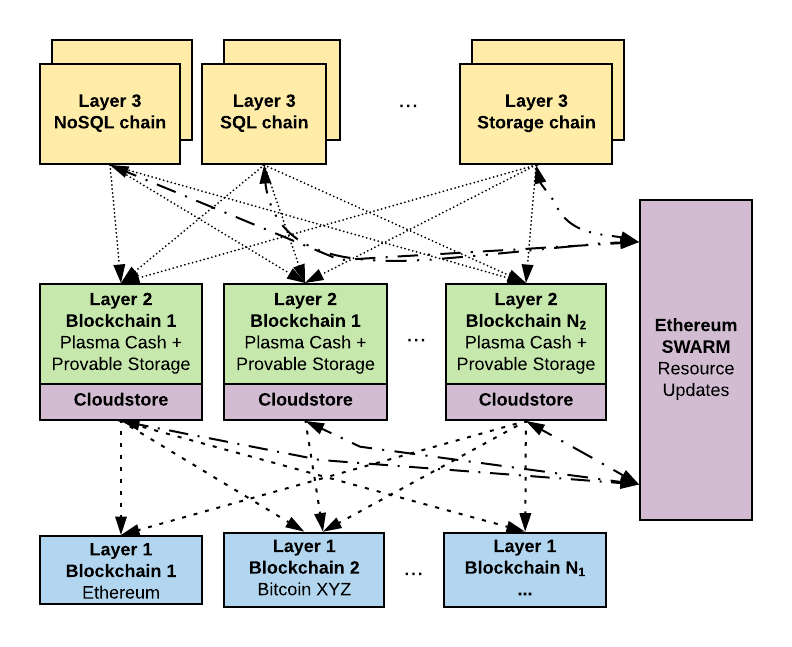
\includegraphics[width=12cm]{DeepBlockchain2.png}} \\
\end{tabular}

\noindent Because the retrieval of layer $i+1$ data from layer $i$ can be verified by layer $i+1$ (checking block data: does the block hash match the block content?  is it signed?  does it have a parent hash? etc.; checking chunks: does the hash of the chunk data equal the chunk key), each lower layer node devolves into a dumb storage layer with some failure or attack probability ($p^2_{1}..p^2_{N_2}$ for layer 2 blockchains, $p_1^{1}..p^1_{N_1}$ for layer 1 blockchains) -- depending on this probabilistic model, the cost of attack may be divined.   However, it seems most likely that motivated parties would attack the centralized control behind each layer (c.f. via EIP999, mining pools arewedecentralizedyet.com, governments asking the Cloudstore providers to block Layer 2 operator's accounts) -- in this sense the probabilistic independence in concentrated efforts to attack layer 1 and 2 would be highly suspect.   For this reason, our true faith relies in Ethereum SWARM's {\em resource updates} (\cite{swarm}), where chunks may be keyed not by the hash of their content but with a {\em resource key}, which can be used for the block data without an index mechanism; all resource updates are signed so the reader can authenticate.  Ethereum SWARM, because of its use of Kademlia-like protocol, is not naturally as fast as other components in Cloudstore, but kicks in when all Layer 2 blockchains Cloudstore fail or when Layer 1 itself is attacked (via 51\% attacks, or unknown POS failures).   If other decentralized storage services provided similar provable storage as Ethereum SWARM's resource update, so long as Layer 3 blockchain does not go Byzantine, only one answer can surface, making for unstoppable layer 3 blockchains. 
 
The Layer 3 NoSQL and SQL blockchains developed in this paper operated under an assumption that the NoSQL + SQL transactions should be private data secured by an encryption key known only to the operators of the Layer 3 blockchain.   This protects the Layer 3 blockchain from operators of Layer 2 blockchain and any Cloudstore.  However, the same problem as with standard databases (MySQL, MongoDB, DynamoDB, etc.) exists with our current implementation of NoSQL/SQL Layer 3 blockchains: once someone gets access to a Layer 3 blockchain node holding the database encryption key or private key, the entire database is compromised. Therefore, provenance and immutability of the NoSQL/SQL database state changes, as manifested in Deep Merkle Proofs, differentiate a Layer 3 blockchain from standard databases. The small latency incurred with permissioned protocols (RAFT, POA) and negligible cost should be welcomed when provenance and immutability are of paramount concern.  For future work, we will be guided by Objective 2.0, in seeking to maximize the cost of attack.  

Many other Layer 3 blockchains can be constructed using the Layer 2 storage and bandwidth infrastructure: a chain that represents the evolving state of ERC721 tokens, a chain that represents a cryptocurrency exchange where your money can never be stolen, and so forth.  The state of the Layer 3 blockchain is not stored locally but instead kept in Cloudstore with storage and bandwidth costs properly accounted for using the Layer 2 tokens, themselves based on Layer 1.  Layer 3 and Layer 2 nodes are therefore ``light nodes'' in that they can quickly catch up to the latest state by asking the layer 2 and layer 1 blockchains for the most recent finalized block.  This is not possible to do for the Layer 1 blockchain, however.  However, it is possible, and interesting to adapt a Layer 1 blockchain of Ethereum and make it a Layer 3 blockchain.  Computation (Ethereum gas costs) can consume {\em Layer 2 token} balances in state channels along with bandwidth, contract storage can use SMTs mapped to Cloudstore (instead of Patricia Merkle Tries kept in local store) submitted in blocks to the Layer 2 blockchain, and the consensus machinery can be put in a modern sharded Proof-of-Stake framework to achieve high-throughput low-latency ambitions of Ethereum 2.0, with all layer 3 nodes.  The expectation would be that a Layer 3 Ethereum blockchain would have massively lower costs due to rational models of storage and bandwidth.   Other deep blockchain systems can be developed with different computational primitives than the EVM, such as Amazon's Lambda or Apache Hadoop.

We believe that there can be many deep blockchain systems developed with higher layers resting on many Layer 1 blockchains, even to the point where multiple Layer 1 systems are dropped and many more added to provide more or less Layer 2 security.  The same can be said for any layer to benefit higher layers.  If the blockchain at layer $i$ changes its consensus algorithm from Quorum RAFT to pBFT or Casper Proof-of-Stake, the layer $i+1$ benefits; higher layer blockchains are supervenient on Layer 1, so innovations on Layer 1 are inherited by all deep blockchain systems.  We hope that many deep blockchain systems can explore high throughput low latency scale through some of the design patterns explored here.

\section*{Acknowledgements}
This work has been supported by participants in the October 2017 Wolk token sale and has been made possible through the guidance and generosity of Viktor Tron and the Ethereum SWARM team.  

%Sets the bibliography style to UNSRT and imports the 
%bibliography file "samples.bib".
\bibliographystyle{unsrt}
\bibliography{main}

\newpage
\section*{Appendix A - Blockchain and Cloudstore Interfaces}

\begin{lstlisting}
type Block interface {
	Hash() common.Hash
	Root() common.Hash 
	Number() uint64
	Time() *big.Int
	ParentHash() common.Hash
	Transactions() []Transaction
	NumberU64() uint64
	Header() Header
	Body() Body
}
type Header interface {
	Hash() common.Hash
	Number() uint64
	NumberU64() uint64
}
type Body interface {
}
type Transaction interface {
	Hash() common.Hash
}
type Backend interface {
	BlockChain() BlockChain       
	TxPool() TxPool               
	Cloudstore() Cloudstore 
}
type BlockChain interface {
	ApplyTransaction(StateDB, Transaction) error
	HasBlock(common.Hash, uint64) bool
	CurrentBlock() Block
	GetBlockByHash(common.Hash) Block
	GetBlockByNumber(rpc.BlockNumber) Block
	SubscribeChainHeadEvent(ch chan<- ChainHeadEvent) event.Subscription
	ValidateBody(Block) error
	GetBlock(common.Hash, uint64) Block
	StateAt(root common.Hash) (StateDB, error)
	InsertChain(chain []Block) (int, error)
	SetHead(uint64) error
	MakeBlock(common.Hash, uint64, []Transaction) Block 
	Stop() error
}
type StateDB interface {
	RevertToSnapshot(revid int)
	Snapshot() int
	Prepare(thash, bhash common.Hash, ti int)
	Commit(Cloudstore) (common.Hash, error)
}
type TxPool interface {
	SubscribeTxPreEvent(chan TxPreEvent) event.Subscription
	Pending() (map[common.Address]Transactions, error)
	Stop()
}
type PendingStateEvent struct{}
type NewMinedBlockEvent struct{ Block Block }
type ChainHeadEvent struct{ Block Block }
type TxPreEvent struct{ Tx Transaction }

type Cloudstore interface {
	RetrieveChunk(k []byte) (v []byte, err error)
	StoreChunk(k []byte, v []byte) (err error)
}
\end{lstlisting}

\end{document}
